\section{Experimentation}
\label{sec:experimentation}

This section is just to provide some initial experiments.

\subsection{Grid World with Dead Ends}
First, we implemented a model similar to the classic grid world problem. The agent may move north, south, east, and west in a $w$-by-$h$ grid world. The agent moves successfully with a $0.8$ probability, and fails by moving right or left, each with a $0.1$ probability. At the edges, if the agent cannot move, it remains still.

Throughout the area, dead ends are placed (denoted by ``-'') as well as goal states (denoted by ``+''). In the normal MDP version, dead ends have a reward of $-\infty$, and only have a positive weight of $1.0$ on the transition probability for remaining in the dead end. Goal states have a reward of $1.0$, and all other states have a small penalty of $-0.03$.

In our MOMDP with lexicographic reward function model, we separate the dead ends and goal states into two reward functions. The first reward $R_1$ provides a $0.0$ reward for all states, and a $-1.0$ reward for transitioning to a dead end. The second reward $R_2$ yields a $1.0$ for transitioning to a goal state, and a $-0.03$ for all other states.

We implemented this initial test in Python 2.7. Figures~\ref{fig:seed_1},~\ref{fig:seed_2}, and~\ref{fig:seed_3} show some example output from the model in this domain. Interestingly, it appears to work very well at strictly avoiding dead ends, and then optimizing around the remaining action possibilities.
\begin{figure}[h]
    \centering
    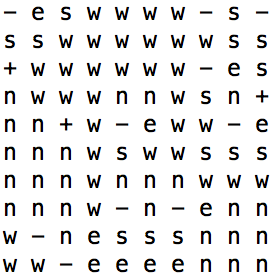
\includegraphics[width=0.4\textwidth,bb=0 0 279 280]{seed_1.png}
    \caption{First example's policy.}
    \label{fig:seed_1}
\end{figure}

\begin{figure}[h]
    \centering
    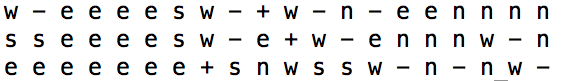
\includegraphics[width=0.4\textwidth,bb=0 0 561 81]{seed_2.png}
    \caption{Second example's policy.}
    \label{fig:seed_2}
\end{figure}

\begin{figure}[h]
    \centering
    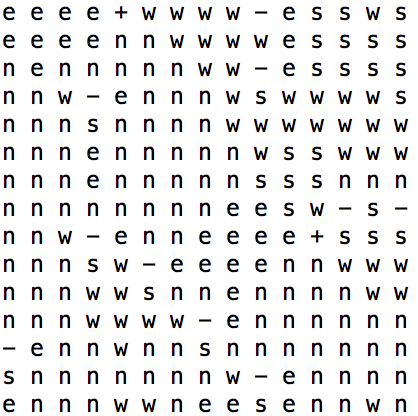
\includegraphics[width=0.4\textwidth,bb=0 0 418 416]{seed_3.png}
    \caption{Third example's policy.}
    \label{fig:seed_3}
\end{figure}

There are additional scenarios for which $\lvmax$ is useful. If there are primary and secondary goals, they can be represented by different rewards, with primary goal states strictly favored over secondary goal states.

\begin{itemize}
    \item If there exists a perfect policy, then it seems to always converge with $\gamma = 1$. The convergent policy always strictly avoids the dead ends, as desired.
    \item Without a perfect policy, it converges but the policy can often be off if a lot of dead ends are close to one another. This is probably one example where the slack variables $\delta_1, \ldots, \delta_k$ could be useful.
    \item These results do not utilize the slack variables: $\delta_1, \ldots, \delta_k$.
\end{itemize}


\subsection{Multi-Objective Autonomous Driving}

To demonstrate the usefulness of both the lexicographic ordering as well as the slack variables, we are considering the autonomous driving domain. We will consider a path planning agent acting over an OpenStreetMap graph, which strictly prefers: shorter time/distance $>$ saving fuel/money $>$ stopping at optional amenities.

Our agent has some slack in optimizing the distance traveled. This allows for it to take an extra 5 minutes to go a bit out of the way in order to save some fuel, or stop at an optional amenity. This same slack holds for the other value functions as well.

We also can model dead ends in this domain. Consider an agent that can choose to drive faster. This might result in a ticket if they drive too fast an get caught, which could be considered a dead end.

This is currently being developed in C++, with supporting scripts to read the OpenStreetMap (OSM) file format written in Python.
